\section{Arquitectura propuesta \label{propuesta}}
\subsection{Selección del modelo de arquitectura\label{arqSelect}}
A la hora de seleccionar la arquitectura, seleccionaremos la que mejor se adapte al casuística de nuestro problema. Por un lado, tenemos la arquitectura Kappa, la cual se reduce a una sola capa donde se procesan los datos y se almacenan para posteriormente mostrarlos en la aplicación. Esto lo podemos ver en la figura \ref{arqKappa} \cite{LambdaKappa2}. Por otro lado, la arquitectura Lambda lanza dos líneas, una para los datos que se han de mostrar rápidamente y otra para los datos de los cuales necesitamos un procesamiento más sofisticado. Esto podemos verlo en la figura \ref{arqLambda} \cite{LambdaKappa}. Vista la casuística del problema se propone, una arquitectura Lambda frente a una arquitectura Kappa.\par

\begin{figure}[htp]
\centering
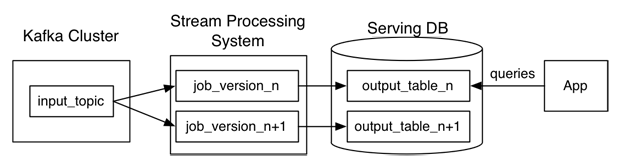
\includegraphics[scale=0.70]{Imagenes/arq1.png}
\caption{Arquitectura Kappa.}
\label{arqKappa}
\end{figure}

\begin{figure}[htp]
\centering
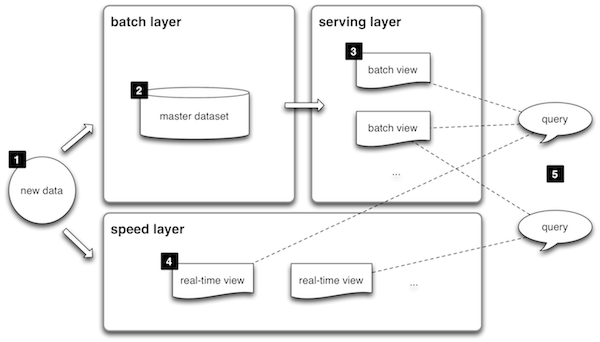
\includegraphics[scale=0.70]{Imagenes/arq2.png}
\caption{Arquitectura Lambda.}
\label{arqLambda}
\end{figure}

\subsection{Selección de las herramientas elegidas\label{toolSelect}}

Debido a la casuística del hardware en el que estamos desarrollando y para conseguir un sistema totalmente portable se ha decidido usar Docker como herramienta para virtualizar los diferentes servicios. De esta forma usaremos menos recursos a la hora de lanzar los diferentes servicios y siendo, aún así, totalmente independientes. Por otra parte con Docker se nos va a permitir encapsular los diferentes servicios para que puedan correrse en cualquier máquina. Aun habiendo elegido este sistema también se ha valorado el uso de un Datacenter Manager como Mesos o Ambari \cite{Hrr-1}, pero resulta ser muy pesado para el hardware que disponemos.\par

Dada la arquitectura seleccionada necesitaremos seleccionar varios tipos de herramientas. Para repartir la carga de los mensajes enviados/recibidos necesitaremos un distribuidor de los diferentes datos que recibamos (broker). Tras recibir el dato necesitamos que la speed layer realice el procesamiento en tiempo real necesitaremos con una tecnología de Streaming que nos permita obtener del dato en bruto, la parte que nos interesa. Por otro lado, la batch layer nos debe permitir almacenar y consultar cualquier dato en cualquier momento ya sea en una o varias bases de datos. Para procesar los datos posteriormente necesitamos un sistema de batching que vaya haciendo resúmenes y obteniendo estadísticas, esto se almacenará en la serving layer. Finalmente, para poder mostrar dichos datos, necesitamos una plataforma de dashboard que nos ayude a mostrar los datos en tiempo real y los post-procesados a la cual, podamos añadir futuros informes.\par

Dicho esto, seleccionamos dos candidatos a brokers que son Kafka y RabbitMQ. RabbitMQ consiste en un sistema de colas tradicional donde encontramos un productor del mensaje y un consumidor del mensaje y diferentes colas a las que se pueden suscribir diferentes productores y consumidores. Por el contrario, Kafka, encontramos que hay un productor del mensaje y varios consumidores del mismo, lo que hace el mensaje persistente hasta un cierto tiempo. Dado que podemos usar también de caché a Kafka para recuperar trabajos y podemos operar fácilmente con las diferentes capas lo seleccionaremos como broker \cite{Hrr-2}.\par

En cuanto a la speed layer encontramos diferentes tecnologías como Spark, Flink o Apex. Spark es un sistema de microbaching, Flink es un sistema de streaming puro y Apex es una nueva tecnología de streaming que está surgiendo ahora en la Apache Foundation. Dado que Apex es una tecnología que aún no está madura la descartamos y nos tendremos que decidir entre Spark y Flink. Spark trabaja en órdenes de segundos, ya que es microbaching, mientras que Flink trabaja en el orden de microsegundos. Aunque Flink es trabaja con tiempos más pequeños \cite{Hrr-4}, realmente no necesitamos tanta precisión en cuanto al tiempo en streaming lo que nos hace, finalmente, decidirnos por Spark dada la comunidad tan grande que existe entorno a esta tecnología. Por otro lado, todas las librerías que lo componen tienen una variedad más rica en funciones y sus desarrolladores más experiencia, por lo que lo hace la más versátil para nuestro problema \cite{Hrr-3}.\par

En cuanto a la parte de almacenamiento a gran escala de los datos nos decantamos por Hadoop, dada la potencia que tiene y la gran cantidad de usuarios que la usan. Por otro lado, podemos seleccionar varios sistemas para realizar el batching, como son Logstash, que pertenece al stack de elastic, Spark o Hadoop.\par

En cuanto a las bases de datos tenemos la opción de usar Postgre, pero dado que queremos más flexibilidad nos decantamos por ver cómo usar bases de datos NoSQL. Aun así, Postgre tiene una potencia más que suficiente y se puede escalar fácilmente. Por otro lado tenemos MongoDB, la base de datos NoSQL más usada a dia de hoy, lo que la hace una muy buena opción para seleccionarla \cite{Hrr-5}. Después de esta, podemos usar Elasticsearch para almacenar datos, aunque sea un motor de búsquedas. Otras alternativas serían InfluxDB que está optimizada para series temporales y Redis, que nos resultará muy útil en cuanto a velocidad de consulta ya que es una base de datos clave valor que almacena sus datos en memoria y persiste a disco cada cierto tiempo. Evidentemente, la empresa tiene ya sus bases de datos que habrá que integrar con esta estructura por lo que la elección tiene que ser especialmente enfocada para el tiempo real. Aunque Redis podría parecer a voz de pronto la mejor herramienta para estos casos \cite{Hrr-6}, consume mucha memoria de la que actualmente, para realizar esta prueba de concepto, no disponemos. Dado esto, nos enfocaremos en usar Elasticsearch para este caso con su stack de tecnologías de forma que nos permitan mostrar un dashboard de una forma mas rapida.\par

En cuanto a la parte de visualización en tiempo real tenemos varias posibilidades como son Kibana con el stack de Elastic, una web realizada a mano con D3 o Grafana que se integra muy bien con InfluxDB. Dado que hemos elegido Elasticsearch y dada la facilidad de usar Kibana, es la herramienta elegida.\par
